
\chapter{Priprema podataka} % Main chapter title

\label{Priprema_podataka} % For referencing 

\section{Objedinjavanje CAFA3 i novije Svis-Prot verzije}

Iz CAFA3 trening skupa izdvojeni su svi validni proteini ( dužine barem 9, i
azbukom od 20 standardnih aminokiselina). U ovom koraku ne izbacujemo proteine
kraće od 40 AK.

Informacije o Svis-Prot bazi podataka dobijene su iz verzije 2017\_12, iz datoteke
\file{uniprot\_sprot-only2017\_12.tar.gz} preuzete sa
\url{ftp://ftp.uniprot.org/pub/databases/uniprot/previous_releases/release-2017_12/knowledgebase}.
Pomenuta verzija sadrži 556 196 proteina. 

Od 66 599 validnih CAFA3 proteina 66 530 ima nepromenjen \keyword{primarni
identifikator}. Međutim  69 slogova u Svis-Prot sadrže nedostjuće CAFA3 identifikatore kao sekundarne.
Kao što je navedeno u potpoglavlju \ref{svis-prot} Ovo je posledica dva moguća mehanizma:

\begin{enumerate}
  \item Unifikacija nekoliko CAFA3 proteina pod novi slog.
    Rezultat unifikacije prikazan je na Slici \ref{fig:unifikacija_slogova}. Analizom
    ovih promena uspešno su rekonstruisana svega četri nova Svis-Prot sloga
    koja odgovaraju nedostajućim CAFA3 proteinima. Kako je četri
    suviše mali broj, zbog jednostavnosti nismo ih ubrajali u dalju analizu
    te koristimo samo 66 530 originalnih CAFA3 proteina.

  \begin{figure}[th]
  \centering
  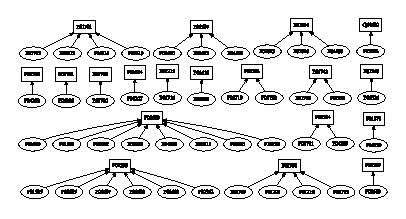
\includegraphics[scale=2]{plots/unifikacija_slogova2.eps}
  \decoRule
  \caption{Unifikacija starih(elipse) na nove slogove u Svis-Prot bazi podataka}
  \label{fig:unifikacija_slogova}
  \end{figure}

  \item Specijalizacija jednog CAFA3 proteina u više različitih slogova.  Zbog moguće
    statističke redundantnosti ovi slogovi su zanemareni.
\end{enumerate}


Validini CAFA3 proteini anotirani su sa  5 957 različitih GO termina Molekulske
Funkcije (MF) od kojih je 50 zastarelo i izbačeno iz \file{go.obo} datoteke.  U
Svis-Prot bazi podataka nismo bili u mogućnosti da proverimo za MF, ali ukupno
je izbačeno 319 GO termina.
CAFA3 sadrži 67 MF koje se ne javljaju u Swis-Prot anotacijama.
Swis-Prot sadrži 888 MF koje se ne javljaju u CAFA3 anotacijama.
Pošto Svis-Prot treba da sadrži svežije (tačnije) informacije, CAFA3 verzija
anotacija je zanemarena u korist novijih Svis-Prot anotacija. Ove informacije
sumirane su  Tabelom \ref{tab:godiff}

Dodatno, Svis-Prot sadrži 194 proteina čija se sekvenca razlikuje u
odnosu na CAFA3 verziju proteina. Odlučili smo da zadržimo originalne CAFA3
sekvence.

\begin{table}[htpb]
  \centering
  \caption{Razlike u GO terminima između CAFA3 i Svis-Prot}
  \label{tab:godiff}
\begin{tabular}{|r|c|c|}
  \hline
                  & CAFA3 & Svis-Prot       \\
  \hline
  MF termini      & 5 957 &    proveriti    \\
  fali u obo.go   & 60 MF & 319 MF, CC i BP \\
  jedinstvenih MF & 67    & 888             \\
  \hline
\end{tabular}
\end{table}

\section{Grupisanje proteina po GO terminima}

Ako za GO termin A važi \textit{is\_a} B i želimo da diskutujemo o funkciji B
onda, i svi proteini funkcije A trebaju biti pridruženi funkciji B. Anotacije
ključnih reči ovo već podrazumevaju dok za GO ovo nije slučaj. Tek nakon što je
ovo grupisanje odrađeno validno je odbaciti termine koji anotiraju manje od 20
proteina.  Za predloženo grupisanje koristili smo algoritam topološkog
sortiranja.  Ovom metodom dobijeno je 1781\footnote{Bez ovog grupisanja imali
bi samo 1146 MF termina} MF termin sa pridruženih minimum 20 proteina
uključujući i koreni termin (molekulske funkcije). U ovom koraku odabrani su
samo proteini minimalne dužine 40 AK.

\section{Ontologije gena i ključne reči}

U nastavku razmatramo samo ključne reči kategorije \keyword{molekulska
funkcija} i načine na koje ih možemo povezati sa ekvivalentnim MF terminima.
Direktno mapiranje sa \keyword{ključnih reči} na GO
termine nije uvek moguće.  Neke ključne reči (Represor, Cyclin, Activator,
Superantigen, Tumorantigen ...) nemaju odgovarajući GO termin. Od 226
ključnih reči svega 175 ima odgovarajući GO termin. Od preostalih 175
postoji 105 mapiranja na MF termin, 59 na BP
i 11 na CC.  Dakle, za 70 MF ključnih reči ne postoji direktno mapiranje na MF
termine.  Slika \ref{fig:KWtop20dis} prikazuje sva moguća direktna mapiranja
(dobijena iz \file{keywords.txt}) za 20 neuređenih MF ključnih reči pronađenih
u radu \parencite{Xie2007}.  U našoj verziji \file{keywords.txt} Antigen je
izbačen i zamenjen specijalizovanijom podelom. Tri ključne reči nemaju
mapiranje, dve se mapiraju na ćelijske komponente, osam na biološke procese i
svega šest na molekulske funkcije. Statistički značajne ključne reči su
ljubičaste dok radi kompletnosti navodimo neke njihove specijalizacije i
generalizacije koje su ofarbane sivo. GO termini su predstavljeni manjim
kružićima. 

Za neke BP termine moguće je doći do molekulske funkcije praćenjem veza ''je
deo'' ili ''sadrži''. Međutim od 8 bioloških procesa sa Slike
\ref{fig:KWtop20dis} ovo je moguće samo za Neuropeptid.
\keyword{Cypher} upitom:
\begin{verbatim}
MATCH p=(:Keyword {name:"Neuropeptide"})--(:GOTerm)<-[*0..]-(:GOTerm)<--(:Protein)
RETURN p
\end{verbatim}
pronašli smo mapiranje predstavljeno Slikom \ref{fig:neuropeptide}. Nažalost
uočava se da MF termini i ključna reč Neuropeptid sadrže svega 5 zajedničkih
proteina. Mi pretpostavljamo da je to posledica veze ''je deo'' koja ne
podrazumeva kompoziciju (''sadrži'') već samo agregaciju\footnote{ Relacija
agregacije podrazumeva da molekulska funkcija postoji nezavisno od biološkog
procesa za razliku od relacije kompozicije}. Kod pomenutih osam BP termina i njihovih
specijalizacija ne javlja se veza ''sadrži''. Pod pretpostavkom da greška nije
u anotaciji GO termina moramo da zaključimo da ovaj metod nije validan.
Dakle automatsko poređenje moguće je samo za šest od 20 originalnih neuređenih MF 
ključnih reči. Za uređene ključne reči postoji više direktnih mapiranja.

Konačni metod koji koristimo da dopunimo gore poemnuto mapirnaje je
poluautomatski. Od ključnih reči (od intersa) ili njihovih delova napravljen je
regularani izraz oblika:
\begin{verbatim}
  expresion = re.compile( f"({'|'.join(words)})[^ ,.)]*", re.I )
  # re.I znači izjednačavanje malih i velikih slova
\end{verbatim}
Konstruisani regularan izraz iskorišćen je na sledeći način. Prvo se pretražuje
da li ime GO termina sadrži neku reč iz regularnog izraza. Ako ne, pretraga se
proširuje na  sinonime GO termina. Ako ni tu nije pronađena, pretraživanje se
proširuje na definiciju termina. Rezultat su tri vrste relacije opadajuće
pouzdanosti (ime, sinonim, definicija). Zajedno sa originalnim direktnim
mapiranjima, pažljivom ručnom analizom moguće je dopuniti mapiranje i izvesti
porđenje rezultata.  Pomenuto mapiranje vršimo nad statički značajnim uređenim
i neuređenim MF termina.  U slučaju da se ključna reč ne pronađe pretraga se
može izvesti za deo imena ključne reči. Međutim ovaj pristup može dovesti do
netačnog mapiranja. Sasvim je moguće da ključna reč nije pronađena jer
odgovarajući MF termini nisu statistički značajni.  Smatramo da je opisan metod
uspešan zbog konzervativnosti fraza koje tražimo kao i informacije o sinonimima
koje GO termini sadrže.

Ključne reči često imaju karakter '-' koju GO termini izbegavaju. Zamena blanko
oznakom je neophodna za pretraživanje imena, ali ne i za sinonime koji često
zadržavaju '-' karakter.  Uočili smo da većina odgovarajućih MF termina ima ime
oblika: \textit{<ime ključne reči> + activity}.



\begin{figure}[th]
\hspace*{-2.2cm} 
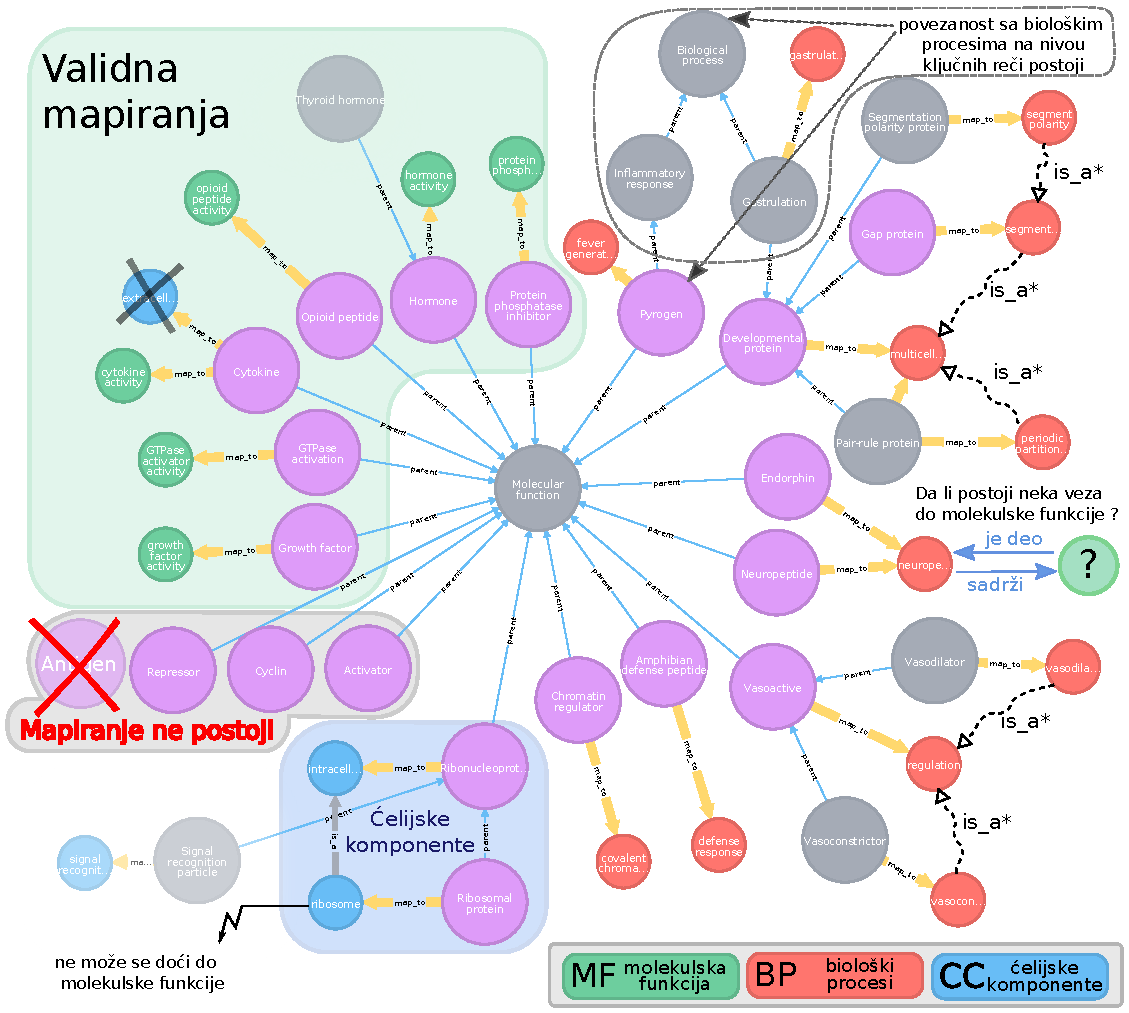
\includegraphics[scale=1]{Figures/plots/kw_dis2go.pdf}
\decoRule
\caption {
  Mapiranje 20 najznačajnijih neuređenih MF ključnih reči \parencite{Xie2007} 
  na GO termine.
}
\label{fig:KWtop20dis}
\end{figure}

\begin{figure}[th]
\centering
\hspace*{-1.0cm} 
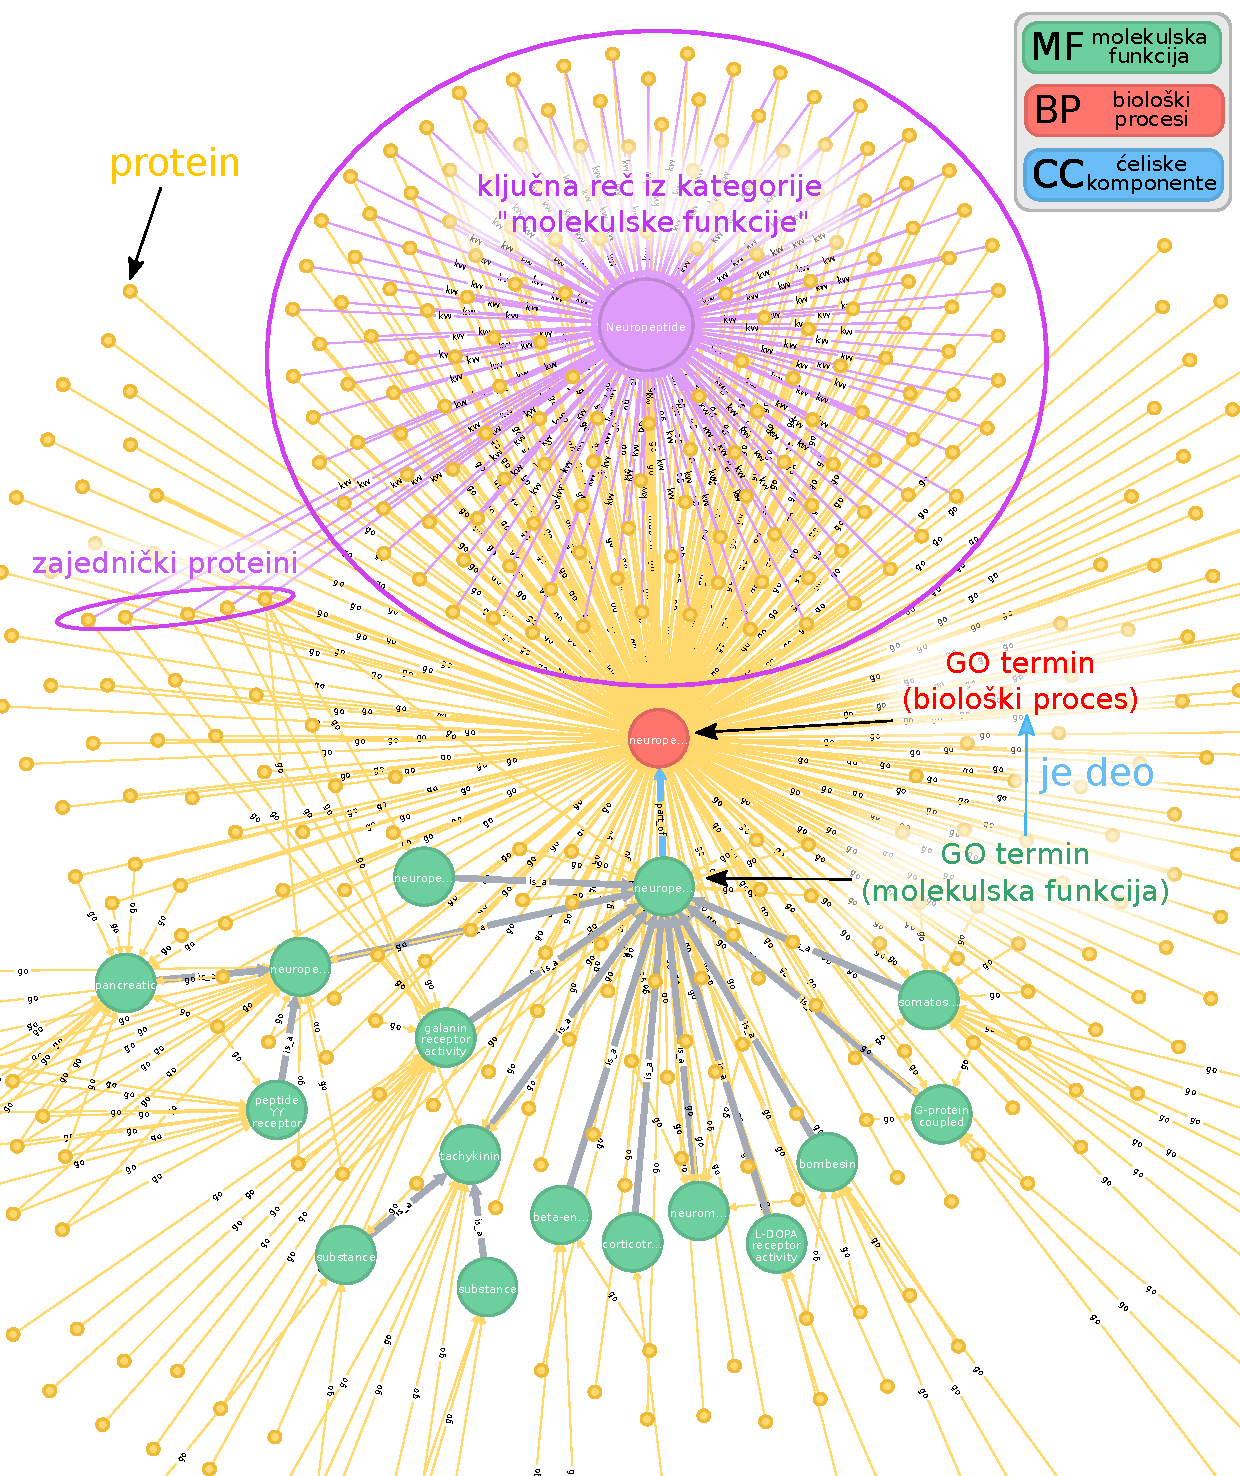
\includegraphics[scale=0.8]{Figures/plots/Neuropeptide2go.pdf}
\decoRule
\caption {
  Mapiranje ključne reči \keyword{Neuropeptid} na MF termine preko veze ''je deo''.
  Ovako postignuto mapiranje rezultuje mali brojem zajedničkih proteina.
}
\label{fig:neuropeptide}
\end{figure}
